% ============================================================
%  K. Kroman, "The Principle of Relativity"
%  Fysisk Tidsskrift, 14. Aargang (1915-16), pp. 1-30.
%
%  ENGLISH TRANSLATION
%  Status: IN PROGRESS. Translated from transcription.tex (the Danish
%  diplomatic transcription, COMPLETE), never from the scan.
%  Structure mirrors transcription.tex 1:1: seven centred roman-numeral
%  divisions I-VII, the same paragraph breaks, the same page markers
%  % --- p. N --- at the same joints, the same footnote anchors.
%
%  RIGHTS: clear. Kroman died 26 July 1925; Danish copyright (life+70)
%  expired at the end of 1995.
%
% ------------------------------------------------------------
%  TRANSLATION CONVENTIONS -- this article
% ------------------------------------------------------------
%  * Standing method: ../../../TRANSLATION-PLAYBOOK.md. Deviations and
%    additions specific to this article are listed here.
%  * QUOTATION MARKS. The Danish sets guillemets »...«; English curly
%    doubles ``...'' here, per the playbook.
%  * EMPHASIS. Every \emph{} run of the transcription is carried over.
%    Where the Danish letterspaces a name and leaves the Danish adjectival
%    suffix outside the run -- \emph{Einstein}'ske, \emph{Newton}'ske --
%    the English keeps the name inside \emph{} and attaches the English
%    suffix outside it: \emph{Einstein}ian, \emph{Newton}ian. Where the
%    printing puts the suffix INSIDE the run (\emph{Doppler'ske} p. 23,
%    \emph{Michelson'ske} p. 30, \emph{Einsteins} p. 29), the whole English
%    form goes inside the run, and a comment marks the spot.
%  * DECIMAL SEPARATOR. Danish decimal commas are set as points in the
%    English (0,02 -> 0.02; 20,5 -> 20.5; 6,4 -> 6.4). Thin-spaced
%    thousands (10\,000) are kept as they are set.
%  * MATHEMATICS is reproduced exactly as the transcription sets it --
%    same \dfrac/\tfrac choice, same case fractions, same displays, same
%    flush-right bare equation numbers via \tag*{}. Nothing is renumbered,
%    resolved or tidied.
%  * THE FIGURE, printed p. 5, is the transcription's TikZ redrawing
%    copied verbatim; its lettering is language-independent. The long
%    comment recording what was measured and what was regularised lives in
%    transcription.tex and is not duplicated here.
%  * PRINTER'S DEFECTS are NOT silently repaired in the translation
%    either. Where a defect is reproducible in English -- p. 4's comma for
%    a full stop -- it is reproduced and marked. Where it is purely
%    typographic in the Danish (a dropped prime, a misplaced apostrophe),
%    the English carries the transcription's reading and a comment.
%  * WORK TITLES stay in their own language (\emph{Das Relativitätsprinzip},
%    \emph{Die neue Mechanik}, \emph{Experimentalphysik}); volume and page
%    references are kept verbatim.
%  * "Stuebevis" (p. 4) -- literally a proof produced indoors, in one room,
%    without astronomical observation. Rendered "indoor proof"; Kroman's
%    point is the parallel with Foucault's pendulum.
%
%  BUILD: pdflatex (libertinus + libertinust1math), like the Danish.
% ============================================================

\documentclass[12pt,a4paper]{article}
\usepackage[utf8]{inputenc}
\usepackage[T1]{fontenc}
\usepackage{libertinus}
\usepackage{libertinust1math}
\usepackage{textalpha}   % Greek in text, typed directly
\usepackage{amsmath}
\usepackage{graphicx}    % for \reflectbox, below
\usepackage{tikz}        % for the redrawn Michelson diagram, printed p. 5
% The old Danish id-est sign »ɔ:« (p. 19) is rendered "i.e." in the English
% per the playbook, so the reflected-c declaration is not needed for the
% body text; it is kept so that the file compiles unchanged if a later
% editor restores the sign in a quotation.
\DeclareUnicodeCharacter{0254}{\reflectbox{c}}

% FOOTNOTES: the printing marks them *), at most one per page. Same fixed
% mark here, at the same anchors.
\renewcommand{\thefootnote}{*)}
\usepackage[english]{babel}
\usepackage{enumitem}
\usepackage[protrusion=true,expansion=true]{microtype}
\usepackage{setspace}
\usepackage[margin=1.2in]{geometry}
\usepackage{fancyhdr}
\setlength{\headheight}{15pt}
\usepackage{hyperref}

\hypersetup{
  pdftitle={The Principle of Relativity},
  pdfauthor={K. Kroman},
  hidelinks
}

\pagestyle{fancy}
\fancyhf{}
\fancyhead[LE,RO]{\thepage}
\fancyhead[RE]{\textit{The Principle of Relativity}}
\fancyhead[LO]{\textit{K. Kroman}}

\setstretch{1.3}

\title{\textbf{``The Principle of Relativity''}}
\author{K.\ Kroman}
\date{\textit{Fysisk Tidsskrift} 14 (1915--16), pp.~1--30\\[2pt]
\small Translated from the Danish}

\begin{document}
\maketitle

% --- p. 1 ---
\begin{center}
I.
\end{center}

It is characteristic of the recent period that several of the more rigorous
sciences have reached such a stage of development that the researchers
concerned have felt themselves prompted to examine more closely the
reliability of the very foundation upon which their science rests. Thus the
mathematicians have for a good many years been occupied with investigations
concerning the foundation of geometry, a labour which, as is well known, has
so far led to the not very gratifying result that even in the mathematical
domain there is no longer agreement among men, since one circle of researchers
maintains that the \emph{Euclidean} basis continues to be the only right one,
while another circle finds it more correct to set up as many as half a score
of different and equally legitimate systems, of which \emph{Euclid}'s is only
one.

In the domain of physics too, relativity endeavours of various kinds have made
themselves felt in recent years. \emph{Newton} was, as is well known, the one
who first clearly and exhaustively set up a general foundation for physics ---
as it was known in his day. But at that time it consisted essentially only of
what we now call mechanical physics. Of the other main divisions of
present-day physics there were as yet but faint traces. Both \emph{Huygens}'
and \emph{Newton}'s optics were still essentially purely mechanical. In our
day there has come in particular an extensive theory of electricity, and with
it there has arisen, among other things, the question: can the manifold
electrical phenomena also be explained on the \emph{Newton}ian basis, or does
this now require additions, indeed perhaps transformations?
% The foot of p. 1 carries the signature line »Fysisk Tidsskrift. XIV.« with
% the sheet number »1« at the outer edge; p. 3 carries »1*«. Signature marks
% are not text of the work and are not transcribed.

% --- p. 2 ---
Owing to the imperfect knowledge we still have of the real nature of
electricity, some time will surely yet pass before a fully grounded answer can
be given to the comprehensive question just mentioned, and it is therefore not
this problem that is to be treated in the following pages. It is rather a
relativity problem of a somewhat narrower kind, namely the \emph{Einstein}ian
hypothesis for the explanation of the \emph{Michelson} light-velocity
experiment, that is to be made the object of a few critical remarks.

A. \emph{Einstein} first presented his views in \emph{Annalen der Physik},
1905, and his treatise has been published, together with several others on the
same subject, in 1913 as a separate little work with the title: H.\ A.
\emph{Lorentz}, A. \emph{Einstein}, H. \emph{Minkowski}: \emph{Das
Relativitätsprinzip}.

The \emph{Einstein}ian hypothesis, which rests chiefly on the presupposition
that it is impossible for us to make any difference between rest and uniform
rectilinear motion, at once aroused considerable attention and met with no
slight adherence; there appeared a fairly luxuriant literature which treated
the problem and sought to carry it further. There were, however, also many who
took a rather sceptical attitude towards his thoughts, and among others both
H. \emph{Poincaré} (in a lecture delivered in Berlin: \emph{Die neue
Mechanik}, issued in a 2nd edition in 1913) and H. A. \emph{Lorentz} (in
\emph{Das Relativitätsprinzip}, 3 lectures, 1914) have expressed particular
doubt as to whether the way out thus indicated can be reconciled with the
fundamental conditions of human knowledge.
% A speck of dirt stands between »antydede« and »Udvej« in the scan; the
% pdftotext layer reads it as a full stop. There is no point on the image.

It seems to me that the eminent researchers named are right in the doubt they
have indicated, and it is therefore especially the \emph{Einstein}ian
hypothesis, seen from the epistemological side, that shall be sought to be
examined more closely in what follows.

\begin{center}
II.
\end{center}

The first occasion of the relativity hypothesis was certain phenomena of
light. The theory of light seems on the whole to be one of the physicists'
problem children. \emph{Huygens} sets up his wave theory; but \emph{Newton}
points out that wave motions can bend round corners, whereas light rays
apparently never do so. Neither could the wave theory manage polarisation,
since for the time being only longitu\-%
% --- p. 3 ---
dinal vibrations were conceived.
\emph{Newton} therefore sets up his emission theory, which wins general
acceptance and holds its ground until it appears that it too leads to
contradictions. The difficulties in the wave theory have meanwhile been
removed, among other things by exchanging the longitudinal vibrations for
transverse ones. Unfortunately, however, vibrations must be vibrations of
something or in something, and one was thereby led to set up that remarkable
``medium'' which is called the ether. It was the elasticity of the ether that
was to maintain the rapid vibrations. One therefore had to ascribe to it an
incredibly great coefficient of elasticity; indeed, since the vibrations were
transverse, one had rather to conceive it as a kind of solid body, while at
the same time one found that it apparently offered the world-globes not the
very slightest resistance. By mathematical means the theory was meanwhile
worked out more and more finely, so that it could by degrees give the most
excellent solution of a multitude of particular problems, and the many elegant
results cast in part a veil over the brittle foundation. An essential advance
took place besides in that \emph{Maxwell} exchanged the elastic vibrations for
electromagnetic ones. The transverse vibrations thereby became explicable, and
the ether lost something of its strangeness. But an enigmatic medium it
nevertheless continued to be under the \emph{Maxwell}ian presuppositions too,
and in its last form as well the theory was soon to lead to apparently
insuperable difficulties.

It had been possible to find the velocity of light in the world-space, in air,
in water and in a multitude of other bodies. One believed further that one had
found a quite simple explanation of the astronomical phenomenon of aberration.
If a telescope is thought of as pointing from the earth straight at the sun, a
light ray which strikes exactly the centre of the objective will not strike
the centre of the eyepiece; for while the light traverses the length of the
telescope, earth and telescope have moved $^{1}\!/_{10\,000}$ of this
% Printed as a case fraction: raised 1, solidus, lowered 10 000 (thin space
% inside the numeral). Kept in that form, not as a built-up fraction.
length to the side, so that the ray will form an angle with the telescope's
axis of about 20.5 seconds of arc. Natural and obvious as this explanation may
seem to be, it nevertheless contains a definite positive presupposition,
namely this, that the light ray retains its direction in space while the
telescope moves to the side, and that the ether, in which the light motion
takes place, thus rests in space and is not dragged along by the earth's
motion. It is the hypothesis of \emph{the resting ether} that is thereby set
up. It is, as one sees, in good agree\-%
% --- p. 4 ---
ment with the circumstance that the globes seem to revolve without suffering
the slightest resistance from the ether.

\emph{Airy} filled a telescope with water and yet obtained through it the
usual aberration constant; this experiment might seem fateful for the usual
theory of aberration, since light takes $^{4}\!/_{3}$ times as long in water
as in air. But it is of course possible, indeed probable, that light cannot
move through water which has a lateral velocity of 30 km per second without
taking along a part of the water's velocity, and if it took, for example,
$^{1}\!/_{4}$ of this, all was of course in order. Now both \emph{Fizeau} and
\emph{Michelson} have shown by experiment that light, in going through water
with a velocity in the direction of the ray, receives a part of the water's
velocity into the bargain. \emph{Fresnel} had, on certain presuppositions
about the ether, predicted that this increment must be
$\dfrac{n^{2}-1}{n^{2}}$ times the water's velocity, $n$ being the water's
% Set as a built-up fraction standing in the run of the line, not displayed.
refractive index. On more recent presuppositions one has come to the same
result, and the experiments of the two researchers fully confirmed this.

The decisive difficulty for current physics therefore first sets in with
A. \emph{Michelson}'s famous experiment. This has already been described in
detail earlier here in this journal\footnote{Vol.\ 10, p.\ 257.}. It will
therefore be sufficient to recall its main points briefly.

\begin{center}
III.
\end{center}

\emph{Michelson}, who was famous for his fine interference experiments,
surely expected by such an experiment to be able to furnish an indoor proof of
the earth's translation, just as \emph{Foucault} by his pendulum and his
gyroscope had furnished an indoor proof of its rotation. He wished, in other
words, to try whether one could not, by the aid of the displacement of the
interference fringes, trace a difference in the time light took to run a
certain relative stretch there and back, when the path fell the one time in
the direction of the earth's translation and the other time stood
perpendicular to it, Since the earth's translation velocity is about 30 km per
% PRINTER'S ERROR, p. 4: the Danish has »vinkelret paa den, Da Jordens« -- a
% comma where the sense and the following capital D require a full stop.
% Reproduced here, comma and capital alike, rather than repaired.
second, thus about a ten-thousandth of the velocity of light in the
world-space and in air, this did not seem to him impossible. He sent out
% --- p. 5 ---
then parallel light rays from $L$, which by the aid of a lightly silvered
plane mirror at $O$ divided, so that some went the one and others the other of
the two paths there and back, whereupon they united again at $O$ and went to
the telescope at $K$. If the relative paths were equally long, the more
absolute ones would of course become different, and the reunited rays would
then have to show a displacement of the interference fringes. His whole
apparatus swam upon mercury and could be turned without coming into
appreciable disorder, so that now the one and now the other set of rays went
the longer of the two paths.

% ================================================================
% FIGURE, printed p. 5.  EDITORIAL REDRAWING IN TikZ -- NOT A FACSIMILE.
% Copied verbatim from transcription.tex, whose comment records what was
% measured off the 600 dpi page image and what was regularised. The
% lettering is language-independent, so nothing here is translated.
% ================================================================
\begin{center}
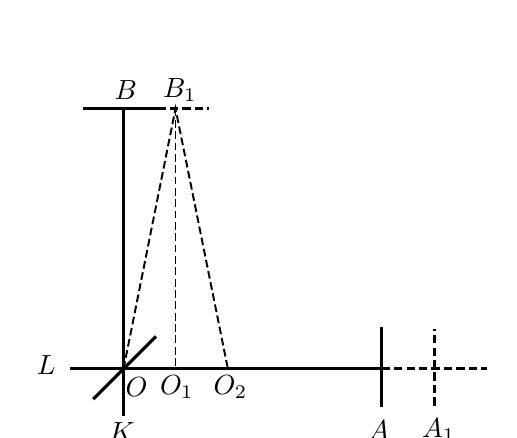
\begin{tikzpicture}[x=0.55cm,y=0.55cm,
    apparatus/.style={line width=1.2pt},
    ray/.style={line width=0.7pt,dash pattern=on 2.8pt off 1.3pt},
    broken/.style={line width=1.2pt,dash pattern=on 3pt off 1.5pt}]

  % --- the base line: the direction of the earth's translation ---
  \draw[apparatus] (-1.24,0) -- (5.96,0);          % L ... O ... A, solid
  \draw[broken]    (5.96,0) -- (8.39,0);           % beyond A, dashed

  % --- the vertical arm, O up to B and down towards the telescope K ---
  \draw[apparatus] (0,-1.10) -- (0,6.01);

  % --- the end mirror at B, and its displaced position at B_1 ---
  \draw[apparatus] (-0.93,6.01) -- (0.78,6.01);
  \draw[broken]    (0.78,6.01) -- (1.97,6.01);

  % --- the lightly silvered plane mirror at O, at 45 degrees ---
  \draw[apparatus] (-0.70,-0.70) -- (0.75,0.75);

  % --- the end mirror at A, and its displaced position at A_1 ---
  \draw[apparatus] (5.96,-0.87) -- (5.96,0.96);
  \draw[broken]    (7.18,-0.85) -- (7.18,0.91);

  % --- the ray's actual path O B_1 O_2, and the perpendicular B_1 O_1 ---
  \draw[ray] (0,0) -- (1.20,6.01) -- (2.41,0);
  \draw[ray] (1.20,6.01) -- (1.20,0);

  % --- lettering ---
  \node[anchor=east]  at (-1.34,0.08) {$L$};
  \node               at ( 0.30,-0.42) {$O$};
  \node               at ( 1.23,-0.42) {$O_{1}$};
  \node               at ( 2.47,-0.42) {$O_{2}$};
  \node               at (-0.04,-1.47) {$K$};
  \node               at ( 0.05, 6.44) {$B$};
  \node               at ( 1.30, 6.44) {$B_{1}$};
  \node               at ( 5.90,-1.42) {$A$};
  \node               at ( 7.28,-1.42) {$A_{1}$};
\end{tikzpicture}
\end{center}

If the earth's motion has the direction $OA$, and if $OA = OB = l$, a light
ray would --- he thought ---, if the earth stood still, take the time
$\dfrac{2l}{c}$ to go there and back between $O$ and $A$ or $B$, $c$ being the
velocity of light. But if the earth itself has the velocity
$v = \dfrac{c}{10\,000}$, the ray which goes to $A$ (which at the same time
comes to $A_{1}$) must take for the outward path the time
$t_{1} = \dfrac{l+vt_{1}}{c} = \dfrac{l}{c-v}$ and for the return path the
time $t_{2} = \dfrac{l-vt_{2}}{c} = \dfrac{l}{c+v}$, thus in all the time
$t = \dfrac{2l}{c}\cdot\dfrac{1}{1-v^{2}/c^{2}}$.

The ray which goes to $B$ will, on account of the earth's motion, traverse the
path $OB_{1}O_{2}$ and must therefore take for the outward path the time
$t_{3} = \dfrac{\sqrt{l^{2}+v^{2}t_{3}^{2}}}{c}$ and for the homeward path the
same time, thus in all the time
$t' = \dfrac{2l}{c}\dfrac{1}{\sqrt{1-v^{2}/c^{2}}}$.

% --- p. 6 ---
The path difference for the two rays thus becomes, to a close approximation,
\[
  F = 2l\left[\frac{1}{1-v^{2}/c^{2}} - \frac{1}{\sqrt{1-v^{2}/c^{2}}}\right]
    = 2l\left[1+\frac{v^{2}}{c^{2}}
      - \left(1+\frac{v^{2}}{2c^{2}}\right)\right]
    = l\frac{v^{2}}{c^{2}} = l\cdot 10^{-8}.
\]
% Displayed, centred, unnumbered; set as one line across the measure.

At \emph{Michelson}'s first experiment\footnote{According to \emph{Wüllner}:
\emph{Experimentalphysik}, 5. Aufl. IV, 607. The numerical magnitudes are
given extremely differently in the various accounts. They play, however, no
essential part in the present connection.} $l = 120$ cm, and the light he
used had the wavelength $\lambda = 60\cdot 10^{-6}$ cm. In a later experiment,
which he carried out together with \emph{Morley}, $l$ had by the aid of
mirrors been increased to 1200 cm. In the first case one obtains
$F = \dfrac{12\cdot 10^{-7}}{60\cdot 10^{-6}}\lambda = 0{.}02\lambda$, in the
last $F = \dfrac{12\cdot 10^{-6}}{60\cdot 10^{-6}}\lambda = 0{.}2\lambda$. One
had then to expect a displacement of the interference fringes of the magnitude
of 0.02 and 0.2 fringe-breadths respectively, now to the one and now to the
other side, according to how the apparatus was oriented. Even the smallest of
these displacements would according to \emph{Michelson} have been observable
in the telescope used, which was furnished with an ocular micrometer. But not
even in the last case was any change with certainty seen in the position of
the fringes.

This negative result was undeniably a surprise, a riddle which brought
contradiction into our physical knowledge. It then became the task to get this
contradiction removed again.

The most obvious way out was both attempted and barred by \emph{Michelson}
himself. He conceived the possibility that the earth at the moment of the
experiment had no real translation either, the whole solar system going at the
same time in the opposite direction with a velocity of 30 km. He therefore
repeated the experiment after the direction of translation had become an
essentially different one. But the result remained as before.

The next nearest way out would be that of declaring the experiment
insufficiently perfect. Where it is only a matter of a path difference of a
fraction of a light wavelength, obviously even the smallest inaccuracies can
destroy the whole thing. Even the very slightest difference of temperature
could of course alter the mutual distance of the mirrors sufficiently. To this
it may however be answered that the distinctness of the interference fringes
and their remaining in place showed decisively
% --- p. 7 ---
that the apparatus was otherwise in order, and that it was expressly the path
difference that it refused to show any sign of.

We must then seek new ways out, and the methodically right course is surely
that we first and foremost turn to the current theory of light itself and ask:
is it then entirely in order? Was one right in expecting the fringe
displacements mentioned?

Here it seems to me that there lies a widely extended field for closer
investigations, a field which surely cannot already be so thoroughly ploughed
that one can give up all searching here and turn to all manner of more remote
possible ways out. As long as interference phenomena have been known, they
have of course caused research surprises which it was only gradually possible
to master. Do we know with sufficient clarity how the luminous bodies go about
producing and emitting the remarkable light vibrations? It is presumably the
general view that light in the world-space and in the atmosphere is constantly
emitted and propagates itself with the constant velocity
$c = 300\,000$ km per second, independently of the light source's rest or
motion. But what secure grounds has this assumption? Might it not be that it
has formed itself rather involuntarily, merely because the possible increments
or deductions that could come into question here seemed so insignificant? It
has been wished to explain \emph{Michelson}'s result by the assumption that
light constantly took along the light source's velocity as an increment.
Objections have been raised against such a view; but against these objections
too objections have been raised. A gentler assumption, however, was that light
in the first moments took along the light source's motion, but quickly passed
over to the usual velocity. That the current theory should be so firmly formed
that there were no room at all for one or the other of such alterations is
surely a hasty belief. Neither is the behaviour of the ether presumably as yet
so firmly established that there should be no room here for one nuance or
another which would make a solution of the riddle possible. A number of
experiments have of course followed \emph{Michelson}'s with closely
corresponding negative results. But the most essential of them have all lain
in the domain of light phenomena, and it therefore seems fairly reasonable
that it ought also to be there that one looks first and foremost for the
redeeming way out.

It looks, however, as if the physicists had already grown weary of searching
here. The first attempt at a solution which won a wider
% --- p. 8 ---
adherence had a far broader basis. It came from H. A. \emph{Lorentz} and was
distinguished in any case by being after all a really \emph{physical} attempt
at a solution.

\emph{Lorentz} thought that it would meet with insuperable difficulties to
conceive the ether as carried along by bodies, and he felt himself likewise
convinced that light constantly has the velocity $c$ through the ether and in
air. He therefore assumed that \emph{Michelson}'s negative result must rest
upon this, that every translationally moved body suffers a contraction in the
direction of the motion just great enough that, among other things,
\emph{Michelson}'s result thereby becomes explicable\footnote{The same way out
was proposed at about the same time by \emph{Fitzgerald}.}. If the translation
velocity is $v$, the body's extension in the direction of translation becomes,
according to the hypothesis,
\[
  a = \frac{1}{\sqrt{1-v^{2}/c^{2}}}
\]
times as small as it was at rest. During \emph{Michelson}'s experiment his
apparatus had of course the earth's translation velocity, $v$. It has thus in
this direction become $a$ times as small. But precisely thereby the two light
paths have constantly become equally long.

\emph{Lorentz} remarks that this hypothesis must indeed at the first moment
awaken some wonder. But on closer consideration it becomes after all quite
natural and obvious. The molecular forces must surely in the last resort be
conditioned by the ether, and it can then be no surprise that they can suffer
the assumed slight change in translation. For it is only an exceedingly slight
change that is in question. The magnitude $a$ is only quite imperceptibly
different from 1. The earth's orbital velocity is about 1800 times as great as
that of one of our express trains, and the earth's diameter is about
12\,800 km. And yet its contraction would amount only to 6.4 cm. That no one
has hitherto noticed that things suffered such a contraction can therefore
cause no wonder.

This is the \emph{Lorentz}ian explanation of \emph{Michelson}'s negative
results. It is distinguished, as has been said, by being a really physical
hypothesis, which in its way really explains what was to be explained.
Several --- among others H. \emph{Poincaré} --- have, however, found it
extremely difficult to assume such a physical contraction, which should be the
same for the most different bodies, provided only
% --- p. 9 ---
these had the same velocity, and, as we shall see, the \emph{Einstein}ian
train of thought is then also directed at explaining the results in question
without the introduction of any real physical contraction, indeed, in
Einstein's own view, without introducing any properly new hypothesis at all.
% »efter Einsteins egen Opfattelse« is NOT letterspaced in the Danish, though
% every other occurrence of the name on pp. 1--10 is. Checked on the image;
% the English follows, and leaves this one occurrence unemphasised.

\begin{center}
IV.
\end{center}

The first impulse to his peculiar attempt at a solution \emph{Einstein} surely
received from the \emph{Lorentz}ian contraction hypothesis; but for the rest
he has gone his own quite particular ways. We shall begin by deriving his
famous formulae without as yet building upon his particular presuppositions.
These formulae can namely be obtained from several different starting points,
and moreover by a quite elementary route, and if we proceed in this way while
for the present keeping to quite ordinary presuppositions, we shall in part
perhaps succeed in getting removed the half-mystical gleam which the formulae
have often enough acquired, and in part the subsequent transition to the
particular \emph{Einstein}ian presuppositions will most clearly let these come
forward in their full peculiarity. In spite of this we shall not need to
remove ourselves very far from his own presentation.

We think of ourselves, then, as having in space two rectangular coordinate
systems, $Oxyz$ and $O'x'y'z'$. At a certain moment they coincide completely;
but the latter has, in relation to the former, a translation in the direction
% X here is upright roman in the printing; on p. 10 the same axis is set
% italic as X'. Both readings kept as printed, in the Danish and here.
of the X-axis with the constant velocity $v$. We can think of a corporeal
world attached to each of the two systems, and assume an observer, A, in the
first and an observer, B, in the second, each with his collaborators furnished
with mechanically perfect clocks and measuring rods. Each of them believes his
own system to be at rest and the other's to be in motion, and they both assume
that light in the world-space and in air has the constant velocity $c$
independently of the light source's rest or motion. It is now a matter of
finding out what, in accordance with their different presuppositions, they
must think about each other.
% The observers A and B are set in upright roman throughout pp. 9--10;
% the geometrical points of the p. 5 figure are italic. As printed.

We may begin with A. He sets up his clocks at different places in his system
and procures for them the same rate and setting by sending out light signals
which are thrown back to the starting point. Let the origins of both systems
reckon the time from the moment of their coincidence, and let us for
convenience assume that all operations take
% --- p. 10 ---
their beginning at this point of time. A thus sends at the time 0 a light
signal from $O$ to the place $L$ at the distance $l$. On the signal's arrival
at $L$ the clock there is thus, according to his presupposition, to be set at
$t_{1} = l/c$, and on the signal's return to $O$ the clock there is to show
$t_{2} = 2l/c$. In this way A seeks to procure for all his erected clocks the
same rate and reading.

B, who believes \emph{his} system to be at rest, goes about it in quite the
same way. He sends, for example, at the time $t' = 0$ from $O'$ a signal along
the $Y'$-axis to a clock at the distance $l$. This is set on the signal's
arrival at $t'_{1} = l/c$, and the clock at $O'$ is set on the signal's return
at $t'_{2} = 2\,l/c$.

This procedure appears, however, to A, who believes B's system to be in
motion, as quite incorrect. He finds that the light must have taken for the
outward path the time
$t_{1} = \dfrac{\sqrt{l^{2}+v^{2}t_{1}^{2}}}{c}$ and for the return path the
same time, thus in all the time
$t = \dfrac{2l}{c}\dfrac{1}{\sqrt{1-v^{2}/c^{2}}}$. But if the magnitude
\begin{equation}\tag*{1.}
  \frac{1}{\sqrt{1-v^{2}/c^{2}}} = a,
\end{equation}
% Bare arabic numeral with a full stop, flush right, as printed; \tag* not
% \tag, which would add parentheses.
is set, A thus finds that B's time-indications must so far be $a$ times too
% PRINTER'S ERROR, p. 10: the Danish sets »maaa« for »maa«. Purely
% orthographic and not reproducible in English; the transcription carries it.
small and his time-units (seconds) $a$ times too great. And for B's light
signals along the $Z'$-axis he comes to the same result.

Along the $X'$-axis, however, the matter becomes more composite. B goes about
it here as before. But A finds that if B sends a signal from $O'$ to a place
on the $X'$-axis at the distance $l$, it must take for the outward path the
time $t_{1} = \dfrac{l+vt_{1}}{c} = \dfrac{l}{c-v}$ and for the homeward path
the time $t_{2} = \dfrac{l-vt_{2}}{c} = \dfrac{l}{c+v}$, thus in all the time
$t = \dfrac{2l}{c}\dfrac{1}{1-v^{2}/c^{2}} = \dfrac{2l}{c}\cdot a^{2}$, and
thus $a$ times as long a time as under the corresponding conditions along the
other axes.

If such a contradiction really took place, B must however --- A thinks ---
quickly have discovered it. For it would then have been impossible for him to
get his clock at $O'$ regulated. It can therefore \emph{not} take place. But
this can only be conceived possible if all $X'$-distances $l$ have in reality
had only the length $l/a$. B's system must thus, on account of its motion,
have contracted, so that it itself and all measuring rods and other bodies in
it which have taken part in the mo\-%
% --- p. 11 ---
tion have become $a$ times as short in the $X'$-direction as they were at
rest. If the measuring rods too are shortened, one understands that B has
noticed nothing and that he has continued to measure the $X'$-lengths
$\dfrac{l}{a}$ as $l$. But if one assumes this contraction, all B's signals
there and back will thus have taken only $a$ times as long a time as
calculated by B, and one then gets everywhere in B's system (at rest in the
system) clocks which go $a$ times too slowly in relation to A's, thus so far
an ordinary A-time and an ordinary B-time.
% »Men antager man...« is NOT indented in the printing, but the line above it
% is justified to the right margin: the same paragraph running on, not a new
% one with a dropped indent. Set continuous here too.

This holds, however, only of the clocks' rate.

For with respect to their setting there is for A still something amiss. A
found that the signal in the $X'$-direction must for the outward path take the
A-time $\dfrac{l}{c-v}$. On account of the contraction this must be corrected
to the A-time $\dfrac{l}{a(c-v)}$, thus to the B-time
$\dfrac{l}{a^{2}(c-v)}$. But B had the clock at his distance $l$ set at the
number $\dfrac{l}{c}$. The clock at the B-distance $l$ from $O'$ in the
$X'$-direction is thus set so that it, according to A, gets a deficit of
clock-reading in B-time of
\begin{equation}\tag*{2.}
  u = \frac{l}{a^{2}(c-v)} - \frac{l}{c}
    = \frac{l(c^{2}-v^{2})}{c^{2}(c-v)} - \frac{lc}{c^{2}}
    = \frac{v}{c^{2}}\,l.
\end{equation}

A has thus further found that B's clocks have a deficit of reading
proportional to their $X'$-distances from $O'$. If this distance is negative,
the deficit is negative. At $O'$ it is 0. In system B there is thus for A not
only B-time, but in addition \emph{local time}, much as we here on earth have
not only mean time and sidereal time, but further Greenwich time and local
time or zone time.

Let there now occur some momentary and punctual phenomenon, $F$, which by A
must be referred to the time $t$ and the place $x$, $y$, $z$ and by B to the
time $t'$ and the place $x'$, $y'$, $z'$, and let us determine the relations
between the 8 magnitudes named.

According to the foregoing we can at once set
\begin{equation}\tag*{3.\quad 4.}
  y = y' \qquad\qquad z = z'
\end{equation}
% Two equations on one line share one flush-right tag, printed »3. 4.«.
Further it is easily seen that we must set
\begin{equation}\tag*{5.}
  t = a\left(t' + \frac{v}{c^{2}}\,x'\right).
\end{equation}

% --- p. 12 ---
For if $t'$ is the B-time at the place $x'$, $y'$, $z'$, the parenthesis gives
us the B-time at $O'$, and the A-time is precisely $a$ times as great as this.

In order to get the relation between $x$ and $x'$ we set A's coordinate
$x = m + n$, where $m$ is the distance from $O$ to $O'$ at the A-time $t$,
thus $= vt$ or according to 5
$= va\left(t' + \dfrac{v}{c^{2}}\,x'\right)$, while $n$ is the
$X'$-distance from $O'$ to the phenomenon, thus $x'$ B-metres or
$\dfrac{x'}{a}$ A-metres. We thus obtain, since
$\dfrac{1}{a^{2}} = \dfrac{c^{2}-v^{2}}{c^{2}}$,
% The 1/a^2 equality is a built-up fraction standing in the run of the
% sentence, not a display. As in the Danish.
\begin{equation}\tag*{6.}
  x = a\left(x'\,\frac{v^{2}+c^{2}-v^{2}}{c^{2}} + vt'\right)
    = a\,(x' + vt').
\end{equation}

From 5 and 6 $t'$ is obtained, since one has
\[
  t' = \frac{t}{a} - \frac{v}{c^{2}}\,x'
     = \frac{t}{a} - \frac{v}{c^{2}}\left(\frac{x}{a} - vt'\right);\quad
  t'\,\frac{c^{2}-v^{2}}{c^{2}}
     = \frac{1}{a}\left(t - \frac{v}{c^{2}}\,x\right)
\]
thus
\begin{equation}\tag*{7.}
  t' = a\left(t - \frac{v}{c^{2}}\,x\right).
\end{equation}

And from 6 and 7 $x'$ is obtained, since
\[
  x' = \frac{x}{a} - vt'
     = \frac{x}{a} - avt + a\,\frac{v^{2}}{c^{2}}\,x
     = a\left(x\,\frac{c^{2}-v^{2}+v^{2}}{c^{2}} - vt\right);
\]
\begin{equation}\tag*{8.}
  x' = a\,(x - vt).
\end{equation}

In all one thus obtains
\begin{equation}\tag*{9.}
  \left.
  \begin{array}{l@{\qquad\qquad}l}
    t = a\left(t' + \dfrac{v}{c^{2}}\,x'\right)
      & t' = a\left(t - \dfrac{v}{c^{2}}\,x\right)\\[3ex]
    x = a\,(x' + vt') & x' = a\,(x - vt)\\[1.5ex]
    y = y' & y' = y\\[1.5ex]
    z = z' & z' = z
  \end{array}
  \right\}
\end{equation}
% Two columns closed by one tall right brace, with the number beside it.

As is seen, the one set of formulae is obtained from the other merely by
letting $v$ change sign and changing the unmarked letters into marked ones and
conversely. This is an expression of the fact that B must think exactly the
% »mærkede« / »ikke mærkede« -- Kroman's own idiom for primed and unprimed.
% Kept as "marked" / "unmarked": the sense is plain from the formulae, and
% "primed" would be a modernisation of his vocabulary.
same
% --- p. 13 ---
about A as A thinks about B, apart from the direction of the velocity, and
this we could have predicted, since B of course believed precisely the same
about A as A about B, with the difference named.

From these fundamental formulae a multitude of others can of course be
derived. We shall here merely add further the formulae for the constant
velocity along each of the coordinate axes. If the motion begins at $O$ at the
time 0, one has of course $h_{x} = \dfrac{x}{t}$, $h_{y} = \dfrac{y}{t}$,
$h_{z} = \dfrac{z}{t}$ and of course $h'_{x} = \dfrac{x'}{t'}$,
$h'_{y} = \dfrac{y'}{t'}$, $h_{z} = \dfrac{z'}{t'}$. But then from 9 one
% PRINTER'S ERROR, p. 13: the third of the marked velocities is set »h_z«,
% without the prime; the sense and the two members before it require h'_z.
% Carried over as printed. Verified on the image at 600 dpi.
obtains
\[
  h_{x} = \frac{a(x' + vt')}{a\left(t' + \dfrac{v}{c^{2}}\,x'\right)}
        = \frac{h'_{x} + v}{1 + \dfrac{v}{c^{2}}\,h'_{x}}
\]
and by the same route on the whole
\begin{equation}\tag*{10.}
  \left.
  \begin{array}{l@{\qquad\qquad}l}
    h_{x} = \dfrac{h'_{x} + v}{1 + \dfrac{v}{c^{2}}\,h'_{x}}
      & h'_{x} = \dfrac{h_{x} - v}{1 - \dfrac{v}{c^{2}}\,h_{x}}\\[5ex]
    h_{y} = \dfrac{h'_{y}}{a\left(1 + \dfrac{v}{c^{2}}\,h'_{x}\right)}
      & h'_{y} = \dfrac{h_{y}}{a\left(1 - \dfrac{v}{c^{2}}\,h_{x}\right)}\\[5ex]
    h_{z} = \dfrac{h'_{z}}{a\left(1 + \dfrac{v}{c^{2}}\,h'_{x}\right)}
      & h'_{z} = \dfrac{h_{z}}{a\left(1 - \dfrac{v}{c^{2}}\,h_{x}\right)}
  \end{array}
  \right\}
\end{equation}

By an easy differentiation the same expressions are obtained for variable
velocities. All the formulae together form what the mathematicians call
``an invariant transformation''.

\begin{center}
V.
\end{center}

All this is however for the present merely a mathematical fantasy. We shall
now try to bring it into relation with reality. First we consider it in quite
the usual way.

A believes his system rests. Let us, in order to get a definite starting
point, \emph{for the present} presuppose that he is right; no one has after
all thought of abolishing the concept of rest outright. Further, both
% --- p. 14 ---
A and B entertain the usual view that light, independently of the light
source's rest or motion, has in the world-space and in air the constant
velocity $c$. Let us also for the present presuppose that this is correct.
Then A regulates his clocks in the manner described. To that we must grant him
a complete right. Further he finds that if B's system has the constant
translation velocity $v$, B cannot rightly regulate his clocks as he does.
They must thereby come to go too slowly, and even if, in order to make B's
behaviour intelligible, one assumes the contraction mentioned, they must
further get local time. These assumptions of A's we must likewise declare
justified on the basis of his presuppositions, which we for the present share.
On the other hand, on the basis of these presuppositions we cannot find B's
proceeding justified. We must maintain with A that B is in error. If A rests,
B cannot rest, when there is the velocity difference $v$ between them. And if
we place ourselves at B's standpoint and believe him to be at rest, we can no
longer believe A to be at rest, but must then declare A's whole proceeding
unjustified. Possibly they are both wrong. But the decisive thing is that we
cannot at one and the same time give them both right. Their starting points
cannot be reconciled with each other. Their results stand in contradiction
with each other.

\emph{Einstein}'s view is however quite another. He too builds upon the
above-mentioned presupposition about the velocity of light. But he adds to it
the \emph{new} presupposition that the optical (electrodynamic) phenomena
``like the mechanical ones'' take place in the same way, whether they are
referred to a system at rest or to a system with uniform translation. It is
this presupposition that he calls ``the principle of relativity''. By the aid
of it he will explain \emph{Michelson}'s negative results, and in these
results themselves he finds a guarantee of the presupposition's correctness.
His view of A and B therefore becomes this:

A can (according to the relativity presupposition) never obtain certainty that
his system rests. But he can obtain certainty that it has no acceleration, and
if he has assured himself of this, he also has (according to the relativity
presupposition) the right to measure his lengths and regulate his clocks as he
did. He can also obtain certainty that B has the constant relative velocity
$v$, and according to the presupposition of the constant velocity of light he
can then also rightly judge of B's clocks and whole system as he did. But B is
on the
% --- p. 15 ---
other hand also right in his proceeding. For whether he rests or not, provided
only he has no acceleration, he incurs (according to the relativity
presupposition) no error in reckoning himself at rest.

Here, then, there are \emph{two truths}. A is right; for he has no
acceleration. And B is also right; for he has no acceleration either. But this
obviously will not do. There is in logic a fundamental proposition which says:
A is not not-A; contradictions (in the world of things) do not exist, and
contradictions (in the world of thought) are not tolerated. Truth is not
double. Truth is only one. This proposition needs no defence. Every science is
built upon it. \emph{Einstein}'s theory, on the contrary, stands in conflict
with it. Therefore it must be rejected.
% The fixed point for the page map: »Sandheden er ikke dobbelt« stands on
% printed p. 15, as Høffding cites it in Relation som Kategori (1921),
% p. 75 n. Rendered here "Truth is not double."

Of course it has not been clear to \emph{Einstein} that his doctrine was in
conflict with the principle of contradiction. Then he would surely have given
it up. He has believed that the conflict was only apparent. He himself
emphasises that it looks as if there were a contradiction between his two
presuppositions; but --- he adds --- this is not so. In this, however, he is
wrong. The two presuppositions do not admit of being united. One needs only to
ask: what should B have done if he too had himself believed his system to be
in motion (without acceleration)? Should he have maintained his results? Then
the constant velocity of light would of course have been given up. Should he
have reckoned as A did? Then ``the principle of relativity'' would of course
have been given up. The two presuppositions do not admit of being reconciled,
simply because the one says shortly and plainly: light's velocity is $c$,
while the other says: light's velocity is sometimes $c + v$ and sometimes
$c - v$ and sometimes something in between. This difference can be concealed
by one's using different clocks. But it is not thereby out of the world. In
the domain of time either logic does not permit us to believe in two truths.
We can perfectly well believe in both sidereal time and mean time. But we find
it necessary to keep to one of them at a time when we want to compare
velocities.

\emph{Einstein} has surely believed that he could appeal to another logical
proposition in his defence. For logic says further:
\textit{Diversi respectus tollunt omnem contradictionem}. If a matter is seen
from two sides, there is no contradiction in different judgements being passed
about it. A musician can, for example, be \emph{great} as a virtuoso but
\emph{small} as a
% The Latin tag is set in TRUE ITALIC in the printing, not letterspaced --
% the first italic in the article. \textit{} per playbook §2.
% --- p. 16 ---
composer. And in the same way A's proceeding may be right from A's point of
view and B's from B's point of view.

This way out, however, does not hold either. When the two judges of the
musician speak fully out, it will appear that we have here \emph{two different
judgements about two different things}. In that there is no contradiction. A
third party present may quite well hold both judgements to be right and both
judges to be fully competent. But suppose they had both spoken of the musician
as a virtuoso. Then the contradiction would remain standing for the present,
and the third party would get no order into his consciousness until he had
learned, for example, that the one of the judges was unconditionally competent
and the other unconditionally impossible. But \emph{Einstein}'s case is
precisely of the latter kind; we do not get two judgements about two things,
but two judgements about one thing. B's system is contracted, says A. No, says
B. B's clocks go too slowly and have local time, says A. No, says B. What is
the unfortunate third party now to think? \emph{Einstein} has really no other
answer than: both! But with that we have the two truths again.

What is the time? a Bornholmer asks a tourist from London. It is twelve,
answers the man. That agrees, says the Bornholmer; for my clock is just one,
and the mean sun comes into the meridian here just an hour before it comes
into the meridian for Greenwich. --- With that the contradiction is out of the
world. Here too we had merely two judgements about \emph{two} things. But in
this way A and B will never be able to come to agreement. It looks as if
\emph{Einstein} had presupposed that the physicist was only A or B. But the
physicist is unfortunately the third party, who is to procure unity between A
and B, and this unity is impossible. \emph{Lorentz} has hit the theory's
weakness right in the centre when he somewhere hints that it will be bad if A
and B ever come to speak with each other\footnote{Lorentz: Das
Relativitätsprinzip, 22.---23.}.
% The footnote is set plain: neither »Lorentz« nor the German title carries
% letterspacing or italic here, unlike the notes on pp. 4 and 6. Followed.

\emph{Einstein} will perhaps appeal to the fact that he has really done
nothing but describe how the physicists here in the world actually go about
it. Like system B, the earth has of course, according to their view, a
translation $v$. And yet they go about it like B and regulate their clocks by
light signals quite as he does. They must thus also get B-time and local time
of the same kind as B's, and precisely thereby the \emph{Michelson} result
becomes explicable.

% --- p. 17 ---
To this it is however to be remarked that this contention is untenable. The
great majority of our physicists are undoubtedly more or less convinced that
it must after all surely play a certain part whether the light goes in the
direction of the earth's translation or against it, and it is only because
they know at the same time that the exceedingly slight difference which can
hereby arise will in the great majority of cases be far exceeded by the
various imperfections with which almost all our measurements are encumbered
that they disregard it. But in return they are then also perfectly clear that
it is only a greater or smaller approximation, and not the absolute truth,
that they have reached. Besides, no physicist of course contents himself with
the light signals mentioned; every physicist constantly has in addition other
routes by which he seeks to win the most reliable and exact result that can be
attained at all. And finally the \emph{Michelson} result was of course
conditioned neither by any clock rate nor by any clock setting. It admits of
explanation if we assume the \emph{Lorentz}ian contraction hypothesis. But
with \emph{Einstein} the contraction is of course merely a \emph{conjecture}
in A's consciousness, called forth by his endeavour to get coherence into B's'
% PRINTER'S ERROR, p. 17: »B's'« -- a second apostrophe after the s, where
% the sense requires »B's«. Reproduced as printed.
behaviour. Taken as a reality it stands with \emph{Einstein} quite
\emph{without cause}.

Both \emph{Einstein} and most of his adherents have with great zeal
emphasised something which they call \emph{Newton}'s ``principle of
relativity'', and have often expressed themselves as if it were only a
\emph{Newton}ian thought that they had developed further. Here too, however, a
misunderstanding makes itself felt. It is in reality something brand new that
\emph{Einstein} has uttered, different from everything one finds in
\emph{Newton}. \emph{Newton} was not in the least degree a relativist in the
\emph{Einstein}ian sense of the word. He was, as he has himself set it forth
in the introduction to the \emph{Principia}, convinced that there was
something which had to be called absolute rest and absolute motion, and
something which was only relative rest or motion, and he was likewise
convinced that rest and motion were on the whole different states. This, he
thought, our thought compelled us to assume. In rational mechanics we have of
course also constantly been able, clearly and without contradiction, to make a
difference between rest and relative and absolute motion. We have there set up
for these matters an extensive theory which hardly anyone will raise objection
to. In the domain of thought, therefore, all is in order. But in the face of
\emph{the given real case} uncertainty can arise about what we really have
before us, since we,
% The foot of p. 17 carries the signature line »Fysisk Tidsskrift. XIV.«
% with the sheet number »2«; p. 19 carries »2*«. Not transcribed.
% --- p. 18 ---
as \emph{Newton} says, here lack a secure coordinate system. Often we can by
closer investigation reach a decision; but --- he adds --- sometimes it can be
``hard''. That it should ever be simply and plainly impossible he has not
committed himself to asserting. He has thus stated that there was here a
certain --- perhaps provisional, perhaps lasting --- limitation in our
insight. But if anyone had asserted to him that rest and uniform rectilinear
motion were physically one and the same, he would quite certainly have
protested, and evidently with right. The mathematical concept ``the invariant
transformation'' is presumably a particularly valuable mathematical concept.
But one must take care not to misuse it physically in exaggerated
abstractness. When C and D play ball in the cabin of a ship --- it is said
---, everything will go on in the same way independently of whether the ship
lies still or has uniform translation. This is only a half-truth. C or D or
the spectators will perhaps not discover any difference. But the physicist,
who looks more searchingly at the matter, will hardly find the assertion exact
or exhaustive. He will involuntarily conjecture that since a resting and a
uniformly translationally moved body cannot after all be apprehended by
thought as completely one and the same, there must surely also be some
difference in what happens in the two cases. And it will not be difficult for
him to find out that if the ball is struck forward from C to D and back from D
to C, then, if the ship moves, it must go a longer way the one time than the
other, and if the time for both motions is the same, then the ball must
necessarily have been acted upon in different ways by C and D, and one then
also easily finds that to the arm's relative motion the ship's motion is
constantly added, now as an increment and now as a deduction. But from this
alone it is seen sufficiently clearly that the event in its details is
different in the two cases, and that it is only the peculiar interplay of
these different details that makes the final result the same for the
spectators. Here, then, there is both difference and likeness; but the
characteristic thing in the whole matter is this, that we can everywhere find
\textit{ratio sufficiens} for what happens, the one time as well as the other.
The demand of thought, the principle of causality, is under each of the two
conditions unambiguously observed. The two events come to look alike precisely
because the individual members were different from the one time to the other,
precisely because the ball each time \emph{took along the starting
point\-%
% --- p. 19 ---
's velocity as an increment}. The whole matter is therefore here
% The letterspaced run »Udgangspunktets Hastighed med som Tilgift« is broken
% by the page turn in the Danish: »Udgangspunk-« on p. 18, »tets« on p. 19.
% The English break falls at the nearest available point in the same run.
\emph{rational}. With \emph{Einstein}, on the contrary, the ball, i.e. the
% ɔ: -- the old Danish sign for »det er« -- rendered "i.e." per the playbook.
light, does \emph{not} take along the starting point's velocity as an
increment, as he himself expressly emphasises. And yet the phenomenon is to
become the same in the two cases. This is \emph{irrational}. This is again the
two truths, which he believes he can transform into one merely by veiling them
with a couple of formulae that contradict each other to just the right degree.

It is true that with \emph{Newton}, and in ordinary physics generally, there
are certain formulae which can remain the same in the resting and in the
uniformly rectilinearly moved system. But from that one cannot yet conclude
that there is identity between the two cases. A flying bird draws a little
wagon of the mass $m$ forward on the deck of a resting ship. The wagon begins
with velocity 0 at the time 0. It has only inertial resistance and gets the
acceleration $\gamma$. The bird must thus pull with the force $m\gamma$, and
when the velocity has become $\gamma t$ and the way
$\tfrac{1}{2}\gamma t^{2}$, the bird has applied the force $m\gamma$ through
the way $\tfrac{1}{2}\gamma t^{2}$, thus the energy
$\tfrac{1}{2}m\gamma^{2}t^{2}$.
% The halves are printed as small built-up fractions (1 over 2 with a rule),
% not as the case fractions with a solidus used on pp. 3--4. \tfrac keeps
% that distinction, here as in the Danish.

If the ship goes in the same direction as the wagon with the constant velocity
$v$, the \emph{ship} phenomenon may quite well become entirely the same, both
in respect of the wagon's velocity, its acceleration and the action of force
upon it. But the bird must now deliver the force $m\gamma$ through the
path-length $\tfrac{1}{2}\gamma t^{2} + vt$, thus the quantity of energy
$m\gamma vt$ more than before. It is, among other things, only because we so
often in our calculations deal freely with the force without interesting
ourselves particularly in the \emph{source of the force} that everything can
come to look so alike. Anyone who stands outside both situations will also,
with sufficient care, find them different from each other.

\emph{Einstein} has thus not solved the riddle behind the \emph{Michelson}
phenomenon. He has merely moved it over into a couple of formulae, which he
offers us as a kind of magic remedy against it. But he has overlooked that the
medicine here is worse than the disease, that there is also a well-known
formula which runs: the patient died, to be sure; but the fever left him! If
there were a yawning abyss between A and B, then they might possibly live on
happily, each with his own view. But such an abyss there is not, as we shall
see. They must therefore try to come to agreement, just as the physicist must
try to find a single sovereign truth. But towards the solution of that task
\emph{Einstein}
% --- p. 20 ---
has not furnished the slightest guidance. He has not even seen that there was
a task here.

\begin{center}
VI.
\end{center}

Let us consider a couple of \emph{the theory's applications} and see whether
they should bring us into conflict with the view here maintained\footnote{A
mathematical formula can be true or false according as it is put in connection
with the one basis or the other. We here look at the \emph{Einstein}ian
formulae from the \emph{Einstein}ian basis alone.}.
% In the note the letterspaced run stops at »Einstein«; the suffix »ske« is
% set close, exactly as the possessive »'s« is elsewhere. Followed here.

In the first place, then, we find a couple of simple consequences of the
mutually contradictory starting points.

There lies a rod on system B's $X'$-axis from $x'_{1} = 0$ to $x'_{2} = l$. It
thus has for B the length $l$ and is for him at rest, while for A it is in
motion. From formulae 9 we learn what length A must ascribe to it. One has
\[
  x'_{2} - x'_{1} = l = a(x_{2} - vt) - a(x_{1} - vt) = a(x_{2} - x_{1}),
\]
thus
\[
  x_{2} - x_{1} = \frac{l}{a}.
\]

For A it is thus $a$ times as short as for B.

If such a rod lay in the same way in A's system, we should get
\[
  x_{2} - x_{1} = l = a\,(x_{2}{}' + vt') - a(x'_{1} + vt')
    = a(x'_{2} - x'_{1}),
\]
% As printed: the first member inside the parenthesis carries the prime AFTER
% the subscript, »x_2'«, while every other member on the page has it before,
% »x'_1«. The compositor's inconsistency is kept here too.
thus
\[
  x'_{2} - x'_{1} = \frac{l}{a}.
\]

B thus in the same way finds A's rod contracted.

We think at $t = t' = 0$ of a sphere with centre at $O'$ and radius $R$. It
thus has for B the equation
\[
  {x'}^{2} + {y'}^{2} + {z'}^{2} = R^{2}.
\]

But according to 9 one obtains at $t = t' = 0$ the relations $x' = ax$,
$y' = y$, $z' = z$, thus
\[
  a^{2}x^{2} + y^{2} + z^{2} = R^{2}.
\]

% --- p. 21 ---
For A the sphere has thus become an ellipsoid of revolution with the
semi-axes $\dfrac{R}{a}$, $R$, $R$. It too has thus quite correctly received
the contraction, in the direction of the motion, of the body assumed to be in
motion. If it lay in A's system (which it in fact does at $t = 0$, since the
systems coincide at $t = t' = 0$), A would, according to the formulae,
apprehend it as a sphere and B find it contracted. Even this is of course a
little strange. But the formulae thus do their duty. Purely mathematically
there is nothing amiss. If, on the other hand, we think of A and B as equipped
with eyes so perfect that they could \emph{see} whether there was contraction
or not, we stand again in the midst of the contradiction.

Let us take yet another example of the formulae yielding what they are
contrived to yield.

From a light source at $O$ there goes out at $t = 0$ a momentary flash of
light. In virtue of the constant velocity of light $c$ it will spread as a
growing spherical shell which at the time $t$ has the radius $ct$ and is thus
represented by the equation
\[
  x^{2} + y^{2} + z^{2} - c^{2}t^{2} = 0.
\]

Thus it will present itself for A. How does B find it? Since $y = y'$ and
$z = z'$, we need only seek the value of $x^{2} - c^{2}t^{2}$. But
\begin{align*}
  x^{2} - c^{2}t^{2}
    &= a^{2}({x'}^{2} + v^{2}{t'}^{2} + 2x'vt')
     - c^{2}a^{2}\left({t'}^{2} + \tfrac{v^{2}}{c^{4}}\,{x'}^{2}
       + 2t'\,\tfrac{v}{c^{2}}\,x'\right)\\
    &= {x'}^{2}a^{2}\left(1 - \frac{v^{2}}{c^{2}}\right)
     - c^{2}{t'}^{2}a^{2}\left(1 - \frac{v^{2}}{c^{2}}\right)
     = {x'}^{2} - c^{2}{t'}^{2},
\end{align*}
% The inner fractions are set SMALL in the printing, the outer ones at full
% size; \tfrac and \frac keep that distinction, as in the Danish.
thus
\[
  {x'}^{2} + {y'}^{2} + {z'}^{2} - c^{2}{t'}^{2} = 0.
\]

The phenomenon thus becomes the same for B as for A. In B's system too ``the
light has thus had'' the constant velocity $c$.

Some reader or other will perhaps exclaim in impatience: but this can surely
never have come about naturally! No, wholly naturally it certainly has not.
Thought cannot grasp that a point of light should be able to be in two places
at the same time. But the impatience is out of place. For one then forgets
that it is of course merely the mutually contradictory formulae that conjure
the marvel forth. If A and B had the eyes spoken of before, they would quite
certainly, by using them, get
% --- p. 22 ---
another result. But the formulae have thus here too done what they were
contrived for. They have apparently taught us that light can at one and the
same time have the velocity $c$ both in a resting and in a moved coordinate
system. If one is satisfied with the formulae, one has thus here obtained a
``solution'' of the \emph{Michelson} riddle itself.

It will perhaps be objected: but these formulae can also procure us results
which were not thought of when they were set up. Thus they can, for example,
explain to us the phenomenon of aberration. A fixed star sends, for example, a
light ray down along the $Y$-axis in system A. If the axis is positive in the
ray's direction, one then has
\[
  h_{x} = 0, \qquad h_{y} = c, \qquad h_{z} = 0.
\]

If B's system $=$ the earth, one obtains from this, according to 10, for the
latter
\[
  h'_{x} = -\,v, \qquad h'_{y} = \frac{c}{a}, \qquad h'_{z} = 0,
\]
and thus, $\alpha$ being the aberration angle,
\[
  \mathit{tg}\,\alpha = -\,a\,\frac{v}{c},
\]
% »tg« for the tangent, set in italic like a variable; kept as printed rather
% than turned into \tan, here as in the Danish.
a result which is only imperceptibly different from that found by the
astronomers.

This calculation must however impress no one. For it is of course simply the
usual way of deriving the aberration relation that is here repeated. Had we
used two ordinary coordinate systems, we should have got the astronomical
result itself out. Now we have used two somewhat artificial ones. Thereby the
foreign constant $a$ has come into the result. Fortunately it is so near 1
that it does not do much harm. But had it been widely different from 1, it
would have come along all the same. One ought therefore surely to prefer to
explain aberration in the way hitherto used, by the aid of two ordinary
coordinate systems.

But the \emph{Doppler} phenomenon too can be explained by the formulae! A
light ray is sent from $O$ along the $X$-axis in system A. If the state of
vibration at $O$ at the time $0$ was $= U \cos 2\pi n\alpha$, it is at the
time $t$ at the place $x$
% --- p. 23 ---
\[
  u = U \cos 2\pi n \left(t - \frac{x}{c} + \alpha\right).
\]
But it will thus at the time $t'$ at the place $x'$ in B's system be
\begin{align*}
  u' &= U \cos 2\pi na\left(t' + \frac{v}{c^{2}}\,x' - \frac{x' + vt'}{c}
        + \frac{\alpha}{a}\right)\\
     &= U \cos 2\pi na\left(t'\left(1 - \frac{v}{c}\right)
        - \frac{x'}{c}\left(1 - \frac{v}{c}\right) + \frac{\alpha}{a}\right)\\
     &= U \cos 2\pi na\,\frac{c - v}{c}\left(t' - \frac{x'}{c} + \beta\right).
\end{align*}

The vibration number has thus for B, who moves away from the light source with
velocity $v$, become $n_{1} = a\,\dfrac{c - v}{c}\cdot n$, thus very nearly as
``\emph{Doppler}'s principle'' demands.

Here, however, there is if possible even less ground for satisfaction than in
the previous case. For one can of course here maintain that the result is
decidedly incorrect, and precisely as incorrect as one had to expect it on the
basis of the two coordinate systems which, so to say, shrink under each
other's gaze. By the aid of ordinary coordinate systems the
\emph{Dopplerian} result is obtained extremely easily, for example thus: if
% Here the letterspaced run swallows the suffix in the Danish
% (»D o p p l e r's k e«), where on p. 22 the same word was set with the
% suffix close. The English follows: the whole adjective inside the run here,
% the name alone inside it there.
the velocity of light is $c = n\lambda$, there will pass a fixed point on the
ray's path $n$ waves in unit time; but if the point moves with velocity $v$
away from the light source, the velocity of light in relation to the point
becomes only $c - v$, and there will then pass it only
$n_{1} = \dfrac{c - v}{c}\cdot n$ waves in unit time. The original vibration
number is thus multiplied by $\dfrac{c - v}{c}$, while the magnitude $a$ has
nothing whatever to do with the purely rational phenomenon.

That the theory of relativity can thus procure us various fairly correct
results follows simply already from this, that the two coordinate systems in
reality resemble two ordinary coordinate systems a good deal, and that the
formulae in question likewise, on account of the great velocity of light and
the correspondingly slight value of the magnitudes $\dfrac{v^{2}}{c^{2}}$ and
$\dfrac{v}{c^{2}}$, continue to be tolerably usable. If $c = \infty$, all the
formulae would of course pass over into the usual ones.
% --- p. 24 ---

Indeed, one must even expect that in certain cases one will be able to get
still more sensational results by the use of the formulae. For these are
contrived so as to be able to make the enigmatic contradiction in the
\emph{Michelson} phenomenon apparently disappear, and everywhere where they
lead to such an apparent annihilation of a contradiction there is therefore a
certain probability that we stand face to face with the same enigmatic cause
which has also made itself felt in the \emph{Michelson} experiments and those
akin to them. One must however take good care not to see in such results
proofs of the theory's correctness.

Of course it is not entirely excluded either that the formulae may also for
once, by a chance hit, lead to a correct result. Thus it is not easy to decide
how the matter really stands with the following case, which concerns the
velocity of light in flowing water:

Water flows in the $X$-direction with the constant velocity $v$. It is thus at
rest for system B. A light ray is sent in the same direction through it. Its
velocity in resting water is $\dfrac{c}{n} = h'_{x}$, $n$ being the water's
refractive index. But in system A one then obtains, according to 10, to a
close approximation.
% As printed: a full stop, not a colon, before the display. Kept.
\[
  h_{x} = \frac{\dfrac{c}{n} + v}{1 + \dfrac{v}{cn}}
        = \left(\frac{c}{n} + v\right)\left(1 - \frac{v}{cn}\right)
        = \frac{c}{n} + v - \frac{v}{n^{2}} - \frac{v^{2}}{cn}
        = \frac{c}{n} + \frac{n^{2} - 1}{n^{2}}\,v,
\]
thus precisely \emph{Fizeau}'s and \emph{Michelson}'s result.

The reason why one may not here without further ado conclude that one has
before one a phenomenon akin to the \emph{Michelson} interference phenomenon
is this, that here there was of course no contradiction which was removed by
the use of the formulae.

We shall cast yet a glance at a couple of the velocity formulae and the time
formulae, in order to show what we must accept if we accept these formulae.

Some body or other has in system B the $X'$-velocity $h'_{x}$, and system B
itself has the constant velocity $v$. According to all sound sense one should
then expect that the body in system A would have to get the sum
% --- p. 25 ---
of the two velocities. But the formulae bid us assume that the velocity in
system A becomes only
\[
  h_{x} = \frac{h'_{x} + v}{1 + \dfrac{v}{c^{2}}\,h'_{x}}.
\]

Therewith, then, the usual addition of velocities, indeed the whole
parallelogram theorem, is abolished. And here too there is no sense in
consoling oneself with the thought that the difference from the usual is only
exceedingly slight. For this difference is at the same time a difference
between \emph{the comprehensible} and \emph{the incomprehensible}. No one will
after all be satisfied with a theory which declares
$2 + 2 = 4 + \varepsilon$, even if $\varepsilon$ is an ever so small
magnitude.

Nor are the remarkable consequences exhausted with so little. If $h'_{x}$ and
$v$ are both merely a trifle less than $c$, the formulae make $h_{x}$ less
than $c$ as well. For if one sets $h'_{x} = c - \mu$ and $v = c - \nu$, where
$\mu$ and $\nu$ are both positive, while they may otherwise be thought as
small as one pleases, one obtains
% Note the printing's two distinct sorts here: Greek ν (nu) for the small
% positive quantity and italic v for the velocity, side by side in the same
% formula. The distinction is load-bearing and is kept.
\begin{align*}
  h_{x} &= \frac{2c - \mu - \nu}{1 + \dfrac{(c - \nu)(c - \mu)}{c^{2}}}
         = \frac{2c - \mu - \nu}{1
           + \dfrac{c^{2} - (\mu + \nu)c + \mu\nu}{c^{2}}}\\
        &= c\,\frac{2c - \mu - \nu}{2c - \mu - \nu + \dfrac{\mu\nu}{c}}.
\end{align*}

We are likewise compelled to assume that if $h'_{x} = c$, $h_{x}$ also becomes
$= c$, quite independently of how great or small $v$ may be. For one then has
\[
  h_{x} = \frac{c + v}{1 + \dfrac{v}{c^{2}}\,c} = c\,\frac{c + v}{c + v}.
\]

Indeed, if one wishes to bring the absurdity out still a little more strongly,
one may for example try to solve the following problem: let in system A a
point (for example a light signal) at the time 0 run from $O$ out along the
$X$-axis with velocity $c$, and let system B (which of course may itself be a
light signal) likewise have its velocity $v = c$. The point must then
according to all sound
% --- p. 26 ---
sense continue to coincide with $O'$, or in system B get the velocity 0. But
sound sense and the formulae are two widely different things. If one keeps to
the formulae, one gets
\[
  h'_{x} = \frac{c - v}{1 - \dfrac{v}{c^{2}}\,c} = c\,\frac{c - v}{c - v} = c.
\]

The time formulae too lead to the most remarkable results.

We think, for example, of two phenomena, $F_{1}$ and $F_{2}$, which by A must
be referred to the times $t_{1}$ and $t_{2}$ and to the places on the $X$-axis
$x_{1}$ and $x_{2}$. Let $t_{1}$, $t_{2}$ and $x_{1}$ be $= 0$ and $x_{2}$
positive. The two events are thus for A simultaneous. For B they are
determined by the magnitudes $t'_{1}$, $t'_{2}$, $x'_{1}$, $x'_{2}$, of which
$t'_{1}$ and $x'_{1}$ must likewise be $= 0$, while for $x'_{2}$ and $t'_{2}$
one obtains
\begin{gather*}
  x'_{2} = a(x_{2} - vt_{2}) = ax_{2}\\
  t'_{2} = a\left(t_{2} - \frac{v}{c^{2}}\,x_{2}\right)
         = -\,a\,\frac{v}{c^{2}}\,x_{2}
         = -\,\frac{v}{c^{2}}\,x'_{2}.
\end{gather*}

For B the two phenomena thus become, according to the formulae, not
simultaneous. $F_{2}$ comes before $F_{1}$. Simultaneity is thus according to
the formulae something relative. What is simultaneous for one is not so
without further ado for another.

This, for a change, we understand perfectly well. For the simultaneous is here
defined as that which presents itself in like clock readings, and clocks can
as is well known both go and stand differently, just as one must also bear
well in mind that it is one thing that two events are simultaneous, and
another that A or B gets word of them simultaneously. Several relativists,
however, believe they have here made a significant discovery concerning time's
inmost essence.

One has therefore also here become apprehensive, and has with a certain
anxiety asked: but if time is something so relative, might it not be that the
causal relation too showed itself relative, and that the effect merely for the
one came after, but for the other before the cause? It is really not easy to
understand why one has become anxious precisely here; for when one has on so
many other points made existence illogical, one step more could hardly make
much difference. Let us however look at the question!
% --- p. 27 ---

Let for A $F_{2}$ come a little later than $F_{1}$ and be, for example, an
effect of $F_{1}$ at the place $x_{2}$. Can it not then happen that $F_{2}$
for B comes before $F_{1}$, and the effect thereby before the cause?

$F_{1}$ came of course for B as well as for A at the time 0, and for B
$t'_{2} = a\left(t_{2} - \dfrac{v}{c^{2}}\,x_{2}\right)$. If $t'_{2}$ is to
become negative, one must thus have
\[
  \frac{v}{c^{2}}\,x_{2} > t_{2} \quad \text{or} \quad
  \frac{v\,\dfrac{x_{2}}{t_{2}}}{c^{2}} > 1.
\]

Now suppose that $F_{1}$ and $F_{2}$ are a light signal's departure from
$x_{1}$ and arrival at $x_{2}$; then $\dfrac{x_{2}}{t_{2}} =$ its velocity
$= c$, and the condition for $F_{2}$ coming for B before $F_{1}$ will then be
fulfilled if $v$ is greater than $c$.

At this consequence (as well as at a number of other similar ones) one has
however become so alarmed that one has sought to secure oneself by adding to
the two presuppositions already named the further dogma that the velocity of
light $c$ is altogether the greatest velocity to be found in the world. The
more firmly one believes in this assertion, the more firmly will one thus be
able to hope that the effect --- in spite of the two presuppositions --- will
never come before the cause. Now the velocity of light is certainly a great
velocity. But there are nevertheless those who have emphasised that if
gravitation is at all (like every other phenomenon here in the world) a
temporal phenomenon, then it must spread with a velocity many times greater
than that of light.

Someone might here, in support of the doctrine, possibly remark that since we
\emph{necessarily} must rely on the principle of causality and thus assume a
cause before every change, it can be directly concluded from this that $c$
\emph{must} be the greatest velocity in the world. This objection is however
untenable. For the feared consequence proceeds of course solely from the two
mutually conflicting presuppositions. But in assuming them one has broken with
the principle of contradiction, and one cannot then afterwards appeal to the
principle of causality, since these two principles are merely two expressions
for one and the same thing. Here too the formulae have merely done what one
had to expect of them: standing as they do in conflict with the principle of
contradiction, they have also turned the principle of causality upside down.
The mathematical part itself is, as has been said, in order.
% --- p. 28 ---

On the other hand it is, as already remarked, something of an inconsistency
that one is particularly eager to save the principle of causality from
destruction; for the whole theory otherwise reveals but slight respect for the
causal relation. With a rather peculiar example of this we may close these
more special remarks.

Let in the resting system A a man set about travelling around with a certain
velocity, $v$. Of what will then happen \emph{Einstein} reports the following:
the man will then himself become a system B, and his clock will therefore
suddenly set about going more slowly than while he was at rest. When he has
come home again and is at rest, the clock will resume its former rate; but it
will now (if it was originally in order) show somewhat too
little\footnote{Lorentz, Einstein, Minkowski: Das Relativitätsprinzip, 1913,
p. 38.}. Indeed, one has even extended the transformation to hold for the man
himself as well. He will during his motion live a little more slowly than
before, and he will therefore on his homecoming be a little younger than those
of his former contemporaries who stayed at home. It is thus quite simply a
kind of fountain of youth that one has here discovered. It merely has the
defect of being somewhat weak in its action; for according to the formulae the
man will, even if he travels constantly at express-train speed, take a good
10\,000 years to gain 1 second. However, the quantitative interests us less
here. It was the causal relation we wished to examine, and for that it will
already be sufficient to consider the clock a little more closely. Quite of
its own accord this can hardly have adjusted itself at the journey's beginning
to go more slowly, and at its end adjusted itself anew to go as before. And it
would be just as incredible to assume that the man himself should have
adjusted his clock to go wrong as long as he travelled. That B's clocks come
to go more slowly than A's we can, on the presupposition that his system
really moves, understand comparatively easily. For he has of course himself
adjusted them to it by using light signals on the presupposition that he was
at rest. But the travelling man can hardly have ``regulated'' his clock during
his express-train journey by the aid of such signals, on the presupposition
that he was not travelling at all, or that the earth was travelling backwards
under him precisely with the train's velocity. It therefore becomes a
completely causeless phenomenon that \emph{Einstein} has here introduced into
his theory, and moreover a phenomenon which the theory unfortunately in
certain respects has
% The note is set plain: neither »Lorentz« nor the German title is
% letterspaced, as on p. 17. Printed mark *), placed BEFORE the full stop
% (»for lidt*).«) -- unlike the note on p. 29.
% --- p. 29 ---
use for, while it in reality does not follow at all from its presuppositions.

For \emph{Lorentz} the matter would be quite another, just as his theory is on
the whole widely different from \emph{Einstein's}, although the latter's
adherents are also fond of claiming him for their side. \emph{Lorentz} assumes
a real contraction under all motion and has thus a real physical cause to
appeal to. With \emph{Einstein} the contraction is merely a conjecture in A's
consciousness, and that such a thing should be able to alter clocks one can
hardly well believe.
% »E i n s t e i n s« -- the genitive s stands INSIDE the letterspaced run in
% the Danish, unlike the »'s« and »'ske« suffixes elsewhere, which are set
% close. Hence \emph{Einstein's} here, with the possessive inside the run.

\begin{center}
VII.
\end{center}

If we pass from lengths, times and velocities over to accelerations, masses,
forces and so forth, everything becomes doubly fantastic. The formulae's
demands upon our willingness to believe are considerably increased. With full
right \emph{Lorentz} finds it extremely strange that all these wonderful views
have found as rapid an acceptance as they really have. But the explanation of
this phenomenon lies perhaps after all not so very far away. The time was in
reality to no slight degree prepared and suited for a theory like the
\emph{Einstein}ian. For the characteristic thing about this theory is of
course this, that it troubles itself so exceedingly little about causal
connection, about understanding of the whole. If only we can get formulae set
up ``which fit'', and which can therefore procure us information about new
particulars, all is well. If there were a resting ether, it would be able to
become a bad protest against the relativity that has been set up.
\emph{Einstein} is therefore not fond of this assumption, and declares
resolutely: there is no use for an ether.\footnote{Lorentz, Einstein,
Minkowski: Das Relativitätsprinzip, p. 28.} That he at the same time attaches
himself to the \emph{Maxwell}ian theory of light, and thus assumes
electromagnetic vibrations without assuming a dielectric medium which can make
the vibrations in question tolerably comprehensible, does not trouble him. He
has in his theory to no slight degree confused mathematics with physics, and
the same tendency in reality makes itself felt in not a few of the physicists
of the present day.
% Printed mark *), here placed AFTER the full stop (»Brug for.*)«); the note
% on p. 28 places its mark before. Both are kept where they stand.

It was emphasised above that there is a decisive difference between the
\emph{Lorentz}ian and the \emph{Einstein}ian theory. Since both are so often
brought into quite close connection, it will perhaps be in place to state the
difference a little more precisely.
% --- p. 30 ---

\emph{Lorentz} is not a relativist. He assumes a resting ether, and can
already thereby define real rest as rest in relation to the ether. But still
more sharply can he distinguish between rest and translation, in that he
assumes a real contraction under translation. That one cannot \emph{always} in
the real case measure the contraction is a circumstance which does not alter
the matter. \emph{Lorentz} stands so far at the same standpoint as
\emph{Newton}.

\emph{Einstein}, on the contrary, finds the ether superfluous and rejects it.
And he cannot of course with any meaning assume any real contraction, since
his whole doctrine of relativity would thereby be laid in the grave. If there
were contraction, there would of course be a difference between rest and
uniform motion, even if one could not always determine it.

It has been urged: but \emph{Lorentz} and \emph{Einstein} have of course quite
the same formulae in a great multitude of cases. To this it must again be
answered that mathematics is not yet physics. The same mathematical expression
may in two different theories quite well have widely different meaning and
value. When \emph{Einstein}, in the case of the traveller in the A-system,
uses his B-formulae without further ado, he thereby, as has been said,
introduces a physical witchcraft. His B-formulae are here quite unjustified,
since the man has evidently not, like B, regulated his clock by light signals.
When \emph{Lorentz} reckons with the same formulae, there is on the other
hand, in accordance with his presupposition of a real contraction, good sense
in the matter. It therefore seems to me physically confusing when one so often
mixes the two views together by introducing expressions like ``the
Lorentz-Einstein transformation'' and the like, and I see no otherwise than
that one must come to the result that the \emph{Einstein}ian theory, in spite
of all the ingenuity to which it undeniably testifies, must nevertheless in
the end be stamped as a decidedly self-contradictory and thereby impossible
view, while the \emph{Lorentz}ian continues to stand as a possible explanation
of the \emph{Michelsonian} riddle. That this explanation is perhaps not the
final or the best that is to be found has already been intimated. The
\emph{Lorentz}ian contraction too leads of course to various somewhat odd
results: in the face of a velocity $c$ or above, the moved body's volume will
of course become 0 or negative. However, this consequence lies presumably so
far out in the periphery that at all events, as a provisional working
hypothesis, it will be most correct to use the doctrine.
% Three readings on this page in the Danish, all as printed:
%   (a) »M i c h e l s o n'- / s k e Gaade« -- the letterspacing runs on
%       through the suffix, hence \emph{Michelsonian} here, whole word inside
%       the run;
%   (b) »L o r e n t z- / ske Forkortning« -- PRINTER'S ERROR: no apostrophe,
%       and the suffix not letterspaced, where every other occurrence on this
%       page reads »L o r e n t z'ske«. The missing apostrophe is not
%       reproducible in English; the suffix is set outside the run, matching
%       the printing's unspaced »ske«;
%   (c) »Lorentz-Einstein-Transformationen« inside the guillemets is NOT
%       letterspaced, though both names are letterspaced everywhere else.
%       Set plain here too, without \emph.

\begin{center}
\rule{0.16\textwidth}{0.5pt}
\end{center}
% END OF THE ARTICLE. There is no signature, no dateline and no »Fortsættes«:
% the text simply stops, and a short centred tail-piece follows -- a broken
% rule of five graduated dashes, rendered here as a plain short rule.

\end{document}
